\chapter{Entscheidungsbäume}
Der Entscheidungsbaum ist ein Baum mit den Entscheidungen getroffen werden. Das geschieht, indem der Baum von der Wurzel zu einem Blatt traversiert wird. Dabei bestimmt ein Test in jedem inneren Knoten,
mit welchem Kindknoten fortgefahren wird. Jedes Blatt entspricht einer Entscheidung des Entscheidungsbaums. Es wird unterschieden zwischen Bäumen, die versuchen eine der vordefinierten Klassen zu klassifizieren,
und mit solchen, die versuchen den nächsten Wert vorherzusagen.
\newline
\newline
Die Konstruktion eines optimalen binären Entscheidungsbaumes ist NP-Vollständig \cite{laurent1976constructing}. Aus diesem Grund werden bei der Konstruktion
Heuristiken verwendet, die nur lokal die beste Entscheidung treffen. Folglich ist es sehr aufwändig den optimalen Klassifizierer mit Entscheidungsbäumen zu finden. Ensemble-Methoden konstruieren eine Menge von
Klassifizierern, dessen Ergebnisse zusammengefasst werden, um die finale Entscheidung zu treffen \cite{dietterich2002ensemble}.

\subsection{Maximierung des Zuwachses der Klassifizierungsgenauigkeit}
Scikit-Learn bietet viele Parameter an, um den Teilungsprozess bei der Konstruktion zu steuern. Einer dieser Parameter ist \texttt{min\_samples\_leaf}, d. h. die minimale Anzahl an Einträgen der Trainingsmenge
in einem Blatt. Dieser steuert die minimale Anzahl an Einträgen die in einem Kindknoten enthalten sein müssen, nachdem ein Knoten geteilt wurde. Standardmäßig ist der Wert 1. Dadurch entsteht ein sehr fein granularer
Entscheidungsbaum, der viele Blätter mit nur einem Eintrag hat. Das heißt, es wurden Teilungen durchgeführt, die nur zwei Einträge unterteilt haben. Der Zuwachs der Klassifizierungsgenauigkeit ist durch diese
Teilungen sehr gering. Eine Erhöhung in der Blattgröße verspricht, dass Entscheidungsbäume gefunden werden können, die zwar tiefer sind, aber dafür eine bessere Klassifizierungsgenauigkeit pro Vergleich erzielen.
Der Baum kann tiefer werden, da die Grenze des Programmspeichers noch nicht erreicht wurde.
\newline
\newline
Abbildung \ref{fig:msl} zeigt, wie sich der Parameter auf verschieden große Trainingsmengen auswirkt. Betrachtet wird eine Maximalhöhe von 16. Besonders bei großen Trainingsmengen (Abbildung \ref{subfig:msl_big})
kann die Programmgröße mit einer Blattgröße von 8 signifkant sinken, ohne die maximale Baumhöhe zu beeinflussen. Bei kleinen Trainingsmengen (Abbildung \ref{subfig:msl_small}) reduziert bereits bei kleinen Blattgrößen
sich die Programmgröße ebenfalls signifikant. Allerdings wird die maximale Baumhöhe beeinflusst. Besonders bei großen Trainingsmengen wirkt sich der Parameter stärker auf die Programmgröße aus.
Vermutlich, da die Anzahl der Blätter sich signifikant erhöht, je tiefer der Baum ist.
\subfigbox{
\subfigure[Trainingsmengengröße: 1023]{\label{subfig:msl_small}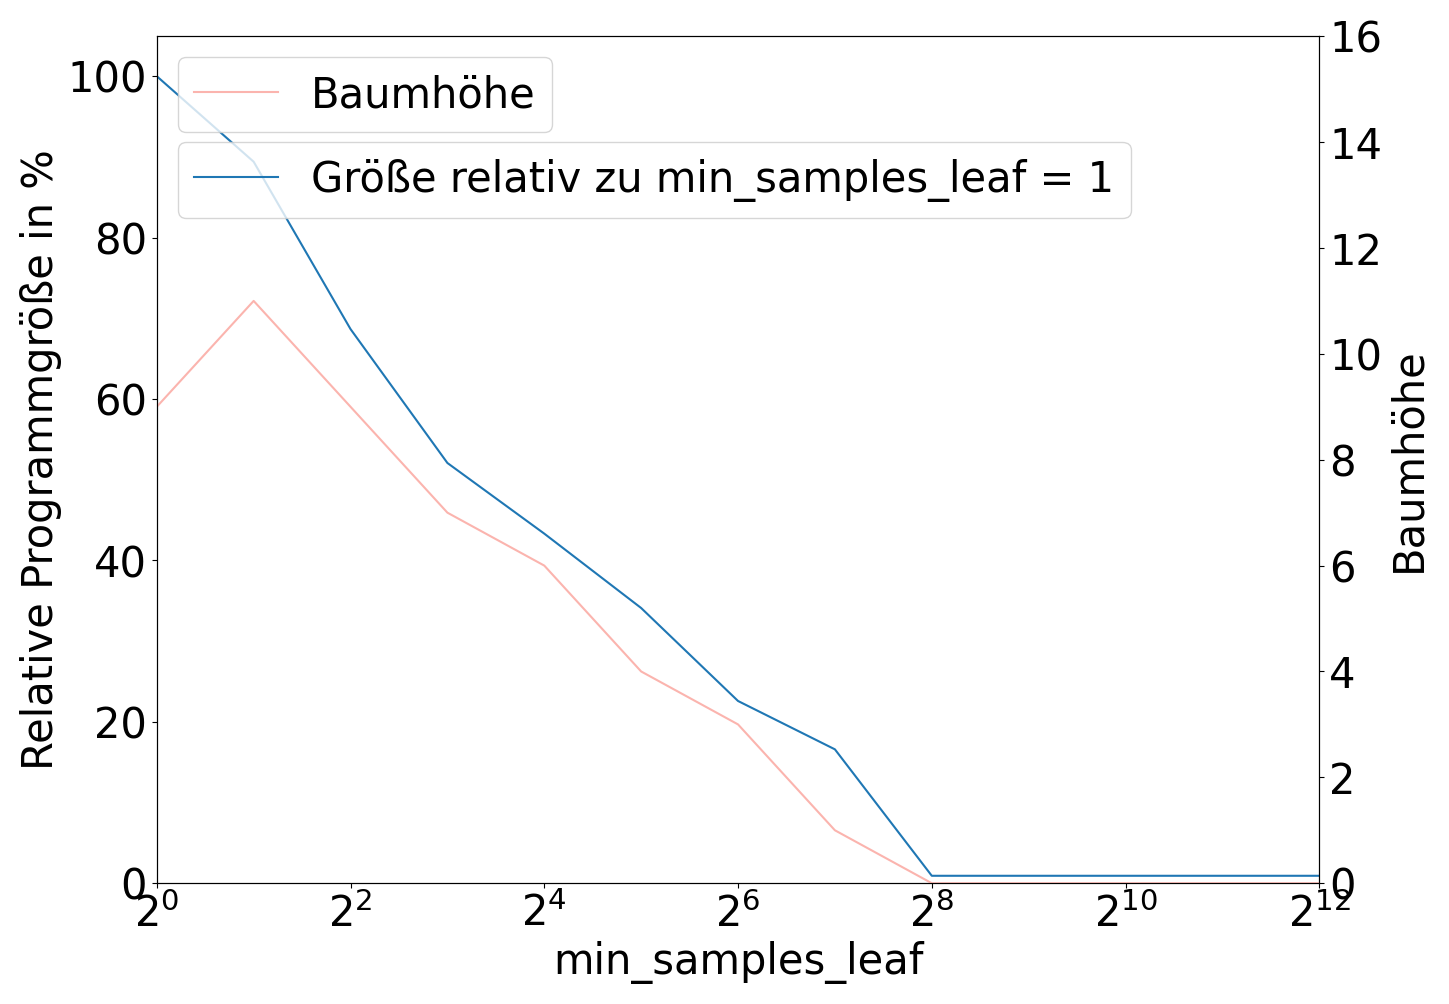
\includegraphics[width=0.48\linewidth]{images/min_samples_leaf_small.png}}\hfill%
\subfigure[Trainingsmengengröße: 7629]{\label{subfig:msl_big}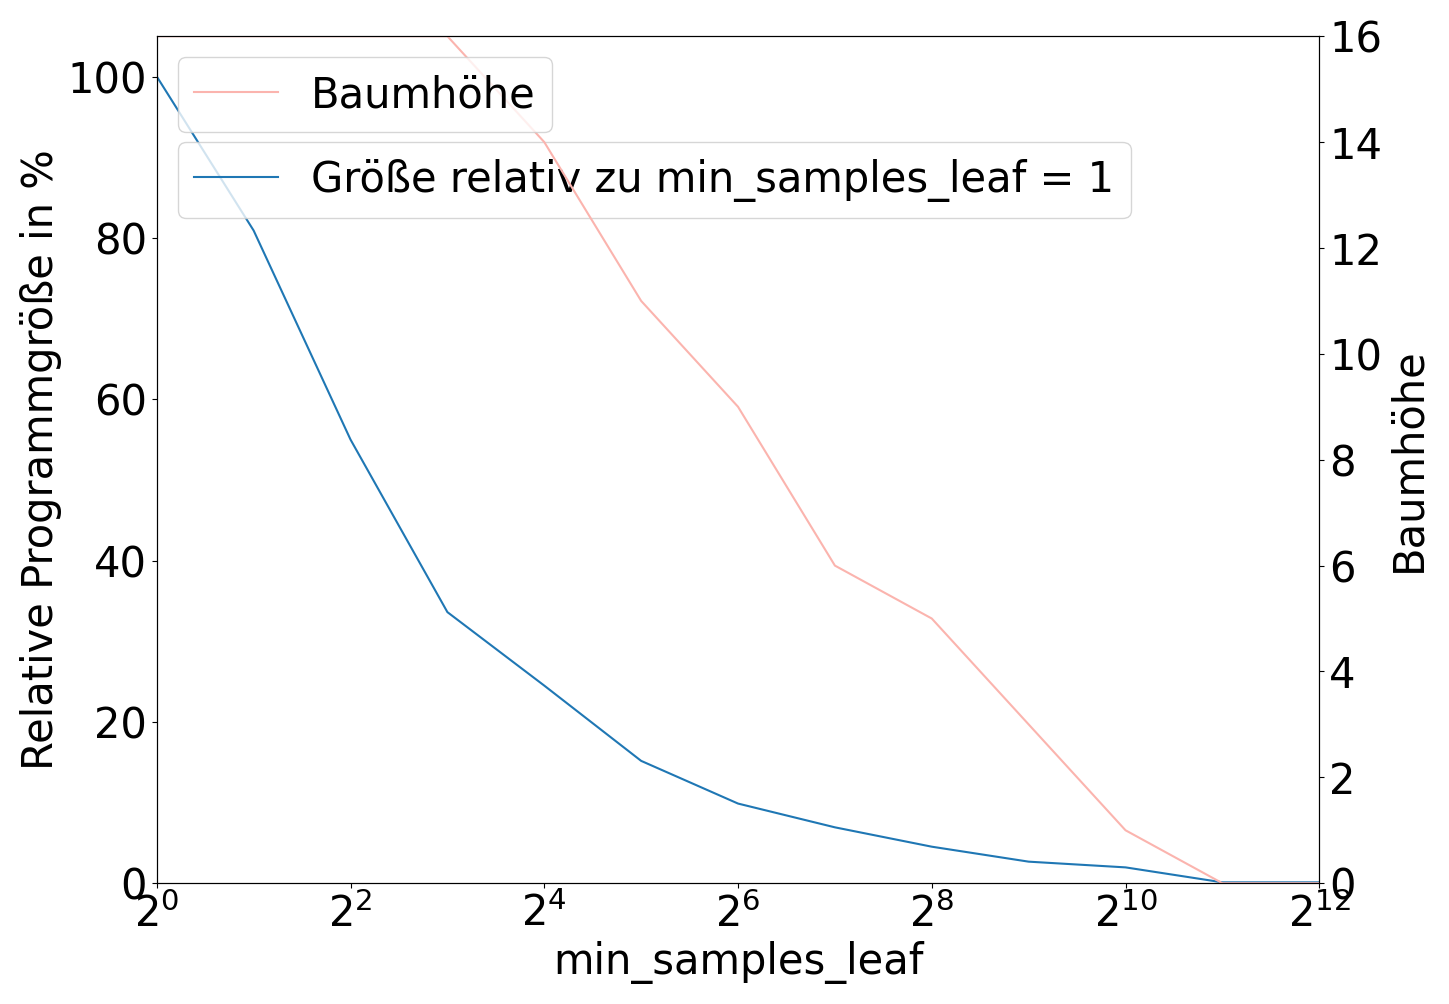
\includegraphics[width=0.48\linewidth]{images/min_samples_leaf_big.png}}%
}{Auswirkung der minimalen Blattgröße auf Programmgröße und Baumhöhe.}{fig:msl}
\newline
\newline
Es kann nicht argumentiert werden, dass ein Wert für die Blattgröße besser ist als ein Anderer, da die Klassifizierungsgenauigkeit auf der Trainingsmenge keine Aussage über die Klassifizierungsgenauigkeit auf
der Testmenge treffen kann. Eine hohe Klassifizierungsgenauigkeit auf Trainingsmenge muss nicht umbedingt eine hohe Klassifizierungsgenauigkeit auf der Testmenge implizieren. Allerdings können so vermeintlich
höhere Entscheidungsbäume ausgewählt werden, da diese weniger Programmspeicher benötigen im Vergleich zu gleich hohen Entscheidungsbäumen mit einer geringeren Blattgröße. Dieser Parameter vergrößert folglich
den Suchraum. Bei kleinen Trainingsmengen ist eine Blattgröße über 1 nur sinnvoll, wenn der größte Entscheidungsbaum, der generiert werden kann, nicht innerhalb der Restriktionen des Programmspeichers liegt.
\section{Entscheidungsbäume}
\begin{figure}
    \centering
    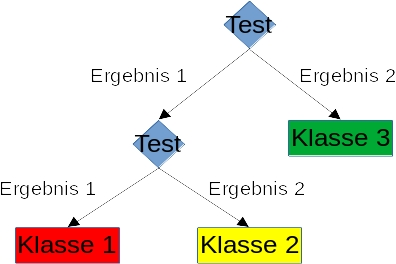
\includegraphics[width=0.5\linewidth]{images/entscheidungsbaum.jpg}
    \caption{Beispiel eines binären Entscheidungsbaums mit 3 möglichen Klassen, die klassifizierbar sind.}
    \label{fig:entscheidungsbaum}
\end{figure}
Der Entscheidungsbaum ist eine rekursive Datenstruktur um Entscheidungsregeln darzustellen. Jedem Blatt ist eine Klasse zugeordnet und allen anderen Knoten ist ein \textit{Test} zugeordnet. Der Test hat eine Reihe von sich
gegenseitig auschließenden Ergebnissen. Die Zuordnung einer Klasse zu einem Objekt wird durch das Traversieren dieses Baumes bestimmt bis ein Blatt erreicht wird \cite{quinlan1990decision}. Abbildung \ref{fig:entscheidungsbaum}
zeigt einen Entscheidungsbaum, wo jeder Test zwei mögliche Ergbnisse hat, i. e. einen binären Entscheidungsbaum. Möglich wäre aber auch das jeder Test eine arbiträre Anzahl an möglichen Ergebnissen hätte.

\subsection{Konstruktion}
\label{sec:construction}
Es gibt viele verschiedene Algorithmen um Entscheidungsbäume zu erzeugen: \texttt{ID3}, \texttt{C4.5}, \texttt{C5}, \texttt{CART}, \texttt{CHAID}, \texttt{QUEST},
\texttt{GUIDE}, \texttt{CRUISE} and \texttt{CTREE}. Am häufigsten wird ID3 (Iterative Dichotomizer 3), bzw. C4.5, welches eine Weiterentwicklung von ID3 ist, und CART (Classification and Regression Trees) verwendet \cite{scikit-learn, singh2014comparative}.
Diese Arbeit verwendet die Implementierung für Entscheidungsbaumklassifizierer von \textit{Scikit-Learn}, die eine optimierte Version von CART nutzt \cite{ScikitLearnCART}. Scikit-Learn ist ein Python-Modul, das eine
große Auswahl von Algorithmen zum maschinellen Lernen implementiert \cite{scikit-learn}.

\subsubsection{CART: Classification and Regression Trees}
Die Konstruktion eines optimalen binären Entscheidungsbaum ist NP-Komplett \cite{laurent1976constructing}. CART ist ein Greedy-Algorithmus, der lokal immer die beste Teilung wählt.
\begin{lstlisting}[label=lst:CARTtreeGrowing,caption={Skizze von vereinfachten Baumwachstumsalgorithmus \cite{steinbergCART}.}]
    Weise dem Wurzelknoten alle Trainingsdaten zu.
    Definiere den Wurzelknoten als Blatt.
    WHILE True:
        Neue_Teilungen = 0
        FOR jedes Blatt:
            IF die Größe der zugewiesenen Trainingsdaten zu klein ist oder alle Einträge der Trainingsdaten zur gleichen Klasse gehören:
                CONTINUE
            Finde das Attribut, das am besten den Knoten in zwei Kindesknoten unterteilt mit einer erlaubten Teilungsregel.
            Neue_Teilungen += 1
        IF Neue_Teilungen == 0:
            break
\end{lstlisting}
Listing \ref{lst:CARTtreeGrowing} skizziert wie CART initial einen maximal großen Baum generiert indem die Trainingsdaten solange geteilt werden bis keine weitere Teilung mehr möglich ist oder alle Einträge der gleichen
Klasse zugeordnet sind. Zuletzt beginnt der Reduzierungsprozess indem Teilbäume gelöscht werden, die die Klassifizierungsgenauigkeit nicht erhöhen oder der Zuwachs unter einem Nutzer definierten
Schwellenwert liegt \cite{steinbergCART}.
\section{Ensemble-Methoden}
Oftmals ist der Suchraum für das Problem zu groß, als das es möglich wäre in tolerabler Zeit die optimale Lösung zu finden \cite{laurent1976constructing}. Konstruktionsalgorithmen für Entscheidungsbäume arbeiten aus
diesem Grund auf Basis von Heuristiken um die lokal optimale Teilung zu bestimmen. Im Gegensatz zu diesen Algorithmen versuchen Ensemble-Methoden nicht die beste Lösung, sondern konstruieren eine Menge von Lösungen
unter denen anschließend gewählt wird, was die finale Lösung für ein Problem ist \cite{dietterich2002ensemble}.

\subsection{Voting}
\subsection{Bagging}
\begin{figure}
    \centering
    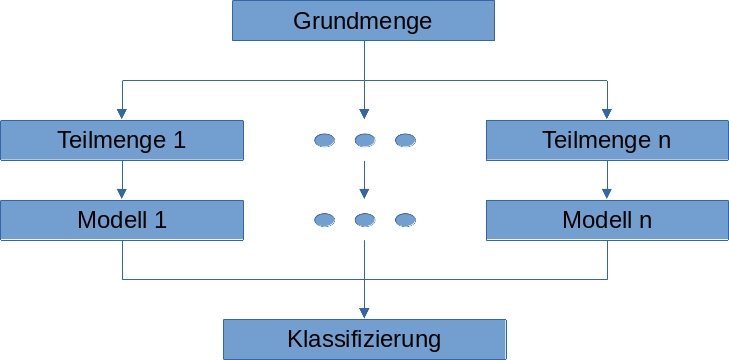
\includegraphics[width=0.6\linewidth]{images/bagging.jpg}
    \caption{Klassifizierungsprozess mit der Bagging-Methode.}
    \label{fig:bagging}
\end{figure}
Bagging ist ein Acronym für \glqq \textbf{B}ootstrap \textbf{agg}regat\textbf{ing}\grqq. Die Idee ist aus einer großen Menge von Trainingsdaten, eine Menge von Mengen von Trainingsdaten zu generieren, folgend mit jedem
dieser Mengen einen Klassifizierer zu trainieren und schließlich alle Klassifizierer, e.g. durch Wählen, zu aggregieren (siehe Abbildung \ref{fig:bagging}) \cite{breiman1996bagging}. Die Methode die dahinter steht nennt
sich \glqq Bootstrap sampling\grqq, welche einen Prozess beschreibt aus einer Grundmenge $m$ mal jeweils $n$ Einträge zu ziehen, die eine Teilmenge bilden \cite{efron1992bootstrap}. Der Name ist folglich aus der Methode
und dem Aggregierungsprozess abgleitet.
\subsection{Random Forest}
Random Forest ist eine Erweiterung der Bagging-Methode. Zusätzlich zu der zufällig ausgewählten Menge an Trainingsdaten wird auch zufällig eine Menge von Features ausgewählt. Auf dieser Basis wird ein Menge von
Entscheidungsbäumen generiert die anschließend aggregiert werden \cite{breiman2001random}.
\subsection{Boosting?}